\chapter{重症支气管哮喘急性发作}

\section{前沿学术综述}

支气管哮喘(简称哮喘)是当今世界威胁公共健康最常见的慢性肺部疾病,其发病率和病死率不断升高。全球至少有1亿患者,其中儿童患病率高于青壮年,老年人群的患病率有增高的趋势。哮喘是一种慢性气道炎症性疾病,这种慢性炎症可导致气道反应性增加,通常会出现广泛多变的可逆性气流受限。哮喘如诊治不及时,随病程的延长可产生气道不可逆性狭窄和气道重塑。因此,合理防治支气管哮喘至关重要。自1995年1月美国国立卫生院心肺血液研究所与世界卫生组织首次发布“全球支气管哮喘防治倡议(global
initiative for
asthma,GINA)”以来,哮喘的防治有了长足的进步,诸如吸入疗法、吸入糖皮质激素(简称激素)为基础的分级阶梯疗法和“六部分综合防治方案”等治疗观点已经得到了哮喘学界的广泛认可。

尽管对哮喘的病理生理日臻了解及治疗药物不断增多,全球支气管哮喘防治倡议方案在我国也开始逐渐推广,但严重的哮喘病例依然较多,病死率仍较高。国内至今尚无全国范围内哮喘病死率的数据,尤其缺乏较长期的纵向研究资料。1999年中华医学会北京分会呼吸专业委员会对北京市16家大医院1988~1998年期间住院哮喘患者资料进行了分析,结果显示10年期间16家医院共收治6410例哮喘患者,且这些患者病情都是较复杂和严重的,其中死亡56例,病死率为0.86%。死亡原因主要有患者发病后就诊过晚,病情重,合并症及伴发病多,以及机械通气时机过晚,也有原来哮喘并不严重,因突发气道阻塞于数小时内死亡者。因此,如何识别重症哮喘并给予恰当的处理,特别是如何有效而安全地使用机械通气,是我们所面临的重要问题。

\subsubsection{哮喘急性发作时严重程度评估}

哮喘急性发作时其程度轻重不一,病情加重可在数小时或数天内出现,偶尔可在数分钟内即危及生命,故应对病情做出正确评估,以便给予及时有效的治疗。哮喘急性发作时严重程度评估见表\ref{tab7-1}。一般而言,重度和危重哮喘均为重症医学科的收治对象。

\begin{table}[htbp]
\centering
\caption{支气管哮喘急性发作的病情严重度分级}
\label{tab7-1}
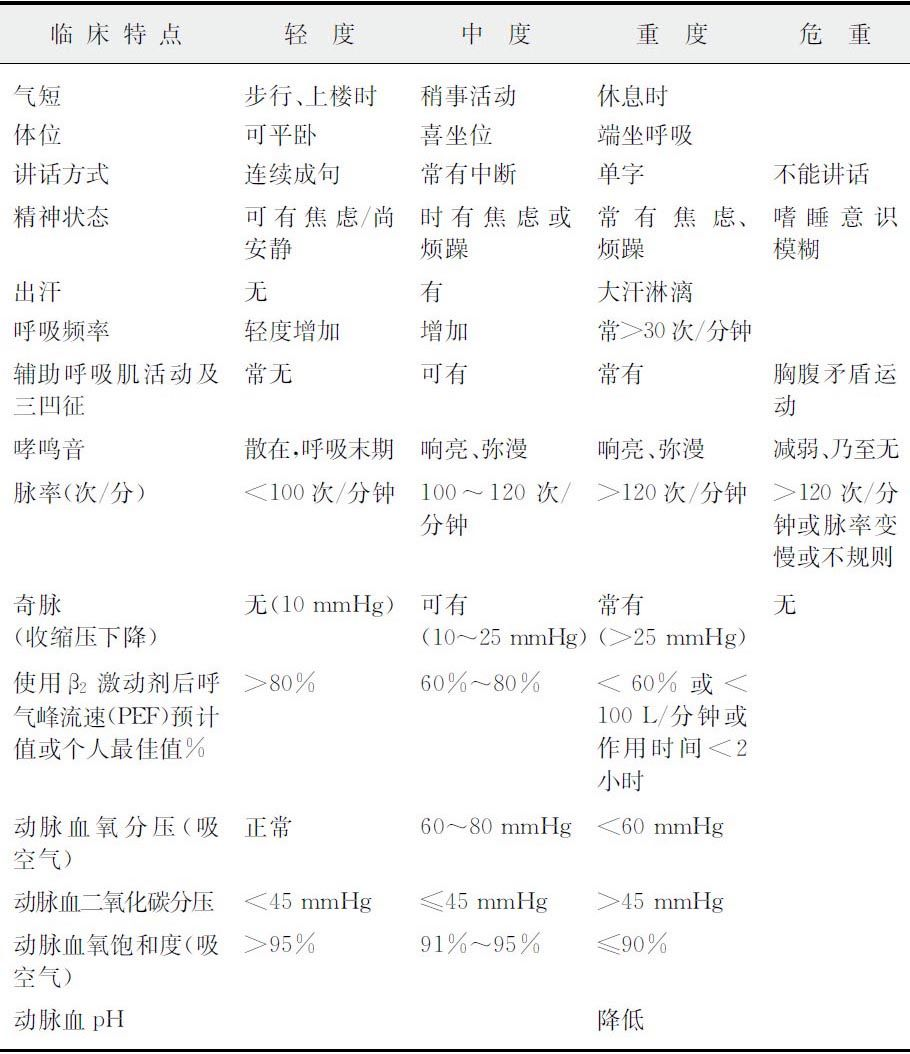
\includegraphics[width=\textwidth,height=\textheight,keepaspectratio]{./images/Image00054.jpg}
\end{table}

\subsubsection{哮喘急性发作药物治疗的进展}

(1)糖皮质激素治疗 糖皮质激素治疗包括全身性应用激素和吸入激素。

糖皮质激素是目前哮喘最有效的抗炎药,能迅速地缓解哮喘的急性发作症状,但全身使用糖皮质激素的不良反应大,故全身用药主要用于中、重度急性发作期哮喘。已有研究显示,糖皮质激素经胃肠道途径与经静脉途径同样能有效控制哮喘的急性发作,一般情况下可口服糖皮质激素。但若患者已有静脉通道或存在胃肠道的吸收功能障碍,可先考虑经静脉途径给药。另外,由于全身性应用糖皮质激素起效较慢(6~12小时)
\protect\hyperlink{text00013.htmlux5cux23ch1-12}{\textsuperscript{{[}1{]}}}
,故需尽早使用。一般而言,与300~400mg/天的氢化可的松等效剂量的糖皮质激素就能有效地缓解哮喘的急性发作症状。而对于哮喘持续状态的患者,推荐静脉使用甲强龙每6小时40~60mg,更大剂量并不能改善预后或使病情更快缓解。哮喘持续状态时急性气道阻塞、气雾剂难以进入气道,故雾化吸入糖皮质激素在治疗哮喘持续状态时的作用仍有异议。而在全身糖皮质激素减量后的数天内,吸入强效的糖皮质激素是有效的。长期口服糖皮质激素后长时间(几周)逐渐减量与短期内逐渐减量相比,无明显优势。2010年全球支气管哮喘防治倡议推荐成人急性发作期哮喘患者口服糖皮质激素治疗时间为7天,儿童为3~5天。

糖皮质激素吸入治疗是重症哮喘患者的有效治疗措施之一,可以有效预防哮喘急性发作和复发,且能达到与口服糖皮质激素相同的疗效。研究显示,哮喘急性发作时,糖皮质激素吸入治疗可以有效改善症状和肺功能,与单纯吸入沙丁胺醇相比,联合吸入糖皮质激素和沙丁胺醇更能有效地扩张气道。虽然糖皮质激素吸入治疗不能完全替代糖皮质激素的全身应用,但对于中、重度的急性哮喘发作患者,高剂量糖皮质激素吸入联合全身性应用糖皮质激素更有助于控制病情,并减少哮喘的急性发作
\protect\hyperlink{text00013.htmlux5cux23ch2-12}{\textsuperscript{{[}2{]}}}
。

定量雾化吸入装置具有成本低、使用方便等优点,因此,可作为糖皮质激素吸入的首选方式。目前没有确切证据表明其他雾化装置的疗效优于定量雾化吸入装置
\protect\hyperlink{text00013.htmlux5cux23ch3-12}{\textsuperscript{{[}3{]}}}
。另外,以氢化氟烷(hydrofluoroalkane)和氟利昂(chlorofluorocarbon)为助推剂的定量雾化吸入装置的治疗效果和安全性相似,但氟利昂可污染环境,所以,临床中应尽量减少以氟利昂为助推剂的定量雾化吸入装置的使用
\protect\hyperlink{text00013.htmlux5cux23ch4-12}{\textsuperscript{{[}4{]}}}
。

(2)短效β\textsubscript{2} 受体激动剂 短效β\textsubscript{2}
受体激动剂是哮喘急性发作期最常用、且起效较快的平喘药。最新全球支气管哮喘防治倡议推荐使用定量雾化吸入装置和储雾罐吸入短效β\textsubscript{2}
受体激动剂。因为在相同药物剂量的条件下,与其他雾化器相比,应用定量雾化吸入装置和储雾罐能更快速控制症状、减少副作用和缩短住院时间。对于不能使用定量雾化吸入装置的患者,如严重呼吸窘迫患者,可考虑使用喷射雾化器,同时用氧气作为气体驱动源,可减少重症患者严重低氧血症的发生。

短效β\textsubscript{2}
受体激动剂持续与间断雾化治疗,对于哮喘急性发作患者的疗效仍有争议。研究显示持续雾化吸入治疗能够增加患者的呼气峰流速并可能降低住院率。另外,对于住院的哮喘急性发作期患者,与较常规的定时(每4小时)雾化吸入治疗相比,按需雾化吸入治疗能降低住院时间和减少短效β\textsubscript{2}
受体激动剂的使用剂量。所以,急性发作期的哮喘患者初始可给予持续的雾化吸入治疗,住院后选择按需雾化吸入治疗较为合适。

虽然已证实长效β\textsubscript{2}
受体激动剂能减少慢性稳定期哮喘患者的急性发作次数,但有关急性发作期应用与疗效的研究还较少。有研究显示福莫特罗和沙丁胺醇类似,具有起效快的特点,且能长时间改善患者的肺功能
\protect\hyperlink{text00013.htmlux5cux23ch5-12}{\textsuperscript{{[}5{]}}}
。另外,有荟萃分析显示
\protect\hyperlink{text00013.htmlux5cux23ch6-12}{\textsuperscript{{[}6{]}}}
,长效β\textsubscript{2}
受体激动剂与吸入糖皮质激素联合应用可能对轻度急性哮喘发作患者有效。关于长效β\textsubscript{2}
受体激动剂在哮喘急性发作中的应用和作用,仍需进一步随机对照研究来证实。

(3)M胆碱能受体阻滞剂 M胆碱能受体阻滞剂可通过降低迷走神经张力而舒张支气管,但其舒张支气管作用较β\textsubscript{2}
受体激动剂弱,起效也较缓慢。2010年全球支气管哮喘防治倡议推荐联用M胆碱能受体阻滞剂和β\textsubscript{2}
受体激动剂雾化吸入治疗急性发作期哮喘患者,因为二者联用较单用更能有效地扩张气道,改善第一秒用力呼气容积和呼气峰流速,且具有起效快,效用时间长和降低住院率等优点。但最近有研究显示,持续雾化吸入M胆碱能受体阻滞剂和短效β\textsubscript{2}
受体激动剂,与单纯持续雾化吸入β\textsubscript{2}
受体激动剂相比,在改善肺功能方面没有显著差异
\protect\hyperlink{text00013.htmlux5cux23ch7-12}{\textsuperscript{{[}7{]}}}
。

(4)茶碱类 茶碱类药物用于支气管哮喘和慢性阻塞性肺部疾病的治疗已有数十年的历史,与短效的β\textsubscript{2}
受体激动剂具有等同的支气管舒张作用。对于轻度急性发作患者,静脉输入茶碱可以显著改善肺功能和缓解呼吸困难症状
\protect\hyperlink{text00013.htmlux5cux23ch8-12}{\textsuperscript{{[}8{]}}}
。传统认为茶碱只具有舒张支气管平滑肌作用,且安全范围小,所以限制了其应用。现在认为茶碱还有其他作用,如抗炎、免疫调节、拮抗腺苷受体、诱导B细胞凋亡、增加膈肌张力、减轻膈肌疲劳等。茶碱的治疗剂量与中毒剂量相近,使用过程中应监测血药浓度。茶碱缓释剂可以维持有效的血药浓度,是理想的茶碱制剂。

(5)硫酸镁 硫酸镁亦具有舒张支气管的作用,但一般不主张对急性发作期哮喘患者常规静脉滴注硫酸镁。最新全球支气管哮喘防治倡议推荐,若出现下列情况可以考虑使用:①第一秒用力呼气量预计值为25%~30%;②对初始治疗无效的成人或儿童;③初始治疗1小时后,第1秒用力呼气量仍未超过预计值的60%。一般可在20分钟内静脉推注2g硫酸镁。

此外,最新的两项系统回顾研究显示,与单用短效β\textsubscript{2}
受体激动剂相比,硫酸镁雾化吸入与短效的β\textsubscript{2}
受体激动剂雾化吸入联合应用,可更有效地改善急性发作期哮喘患者的肺功能并降低住院率,尤其有利于重症哮喘患者的治疗
\protect\hyperlink{text00013.htmlux5cux23ch9-12}{\textsuperscript{{[}9{]}}}
\textsuperscript{,}
\protect\hyperlink{text00013.htmlux5cux23ch10-12}{\textsuperscript{{[}10{]}}}
。

(6)氦氧混合气 氦氧混合气能减少小气道由于狭窄和黏膜表面分泌物增多所引起的湍流发生,从而降低气道阻力,减少呼吸功和氧耗,并有利于二氧化碳排出。可试用于重度哮喘患者。目前主要应用于标准治疗失败的患者。

(7)白三烯拮抗剂 白三烯是引起气道痉挛、气道变应性炎症的介质之一,在哮喘发病中起关键作用。目前已投入临床使用的白三烯拮抗剂主要为其受体拮抗剂(扎鲁司特和孟鲁司特)。每日两次20mg扎鲁司特口服能有效地改善哮喘的症状,并显著改善纤毛摆动
\protect\hyperlink{text00013.htmlux5cux23ch11-12}{\textsuperscript{{[}11{]}}}
。最近一项多中心的随机双盲研究显示,扎鲁司特不仅能改善急性发作期哮喘患者的肺功能和症状,而且能减少急性发作期哮喘的复发率
\protect\hyperlink{text00013.htmlux5cux23ch12-12}{\textsuperscript{{[}12{]}}}
。

(8)其他治疗 主要包括抗生素治疗和黏液溶解剂和胸部物理治疗。哮喘患者一般不常规使用抗生素,当患者出现发热、咯脓痰等细菌感染的征象时才考虑使用。目前没有确切的证据表明黏液溶解剂和胸部物理治疗对急性发作期哮喘有效。

\section{临床问题}

\subsubsection{重症哮喘的主要临床表现有哪些?}

重症哮喘患者的主要临床表现包括:不能平卧,讲话不连贯,烦躁不安,呼吸频率>30次/分钟,胸廓饱满,胸廓运动幅度下降,辅助呼吸肌参与呼吸,心率>120次/分钟,成人的呼气峰流速<100L/分钟,动脉血氧分压<60mmHg(1mmHg=0.133KPa),动脉血二氧化碳分压≥45mmHg,动脉血pH下降。X线胸片表现为肺充气过度,气胸或纵隔气肿。心电图呈肺性P波,电轴右偏,窦性心动过速。病情更危重者会出现嗜睡或意识模糊,胸腹呈矛盾运动(膈肌疲劳),哮鸣音消失。

\subsubsection{如何将支气管哮喘按照其发生呼吸衰竭的方式进行分类?}

某些哮喘患者的肺功能在几天内逐渐恶化,而有些患者在几分钟到数小时内可从正常的肺功能状态下发生哮喘的致死性发作。因此有人将发生急性呼吸衰竭的哮喘分成两类,即急性严重哮喘和急性窒息性哮喘(表\ref{tab7-2})。

\begin{table}[htbp]
\centering
\caption{哮喘按呼吸衰竭的方式分类}
\label{tab7-2}
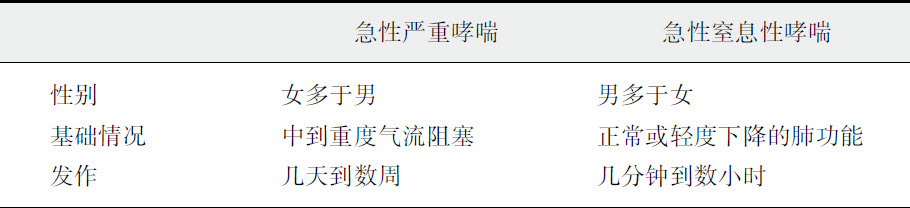
\includegraphics{./images/Image00055.jpg}
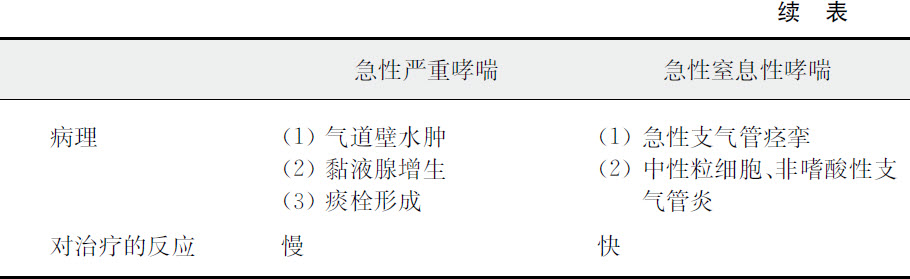
\includegraphics{./images/Image00056.jpg}
\end{table}



\subsubsection{导致重症哮喘的常见病因有哪些?}

重症哮喘形成的原因较多,发生机制也较为复杂,哮喘病人发展成为重症哮喘的病因往往是多方面的。作为临床医生在抢救重症哮喘病人时应清醒地认识到,若要有效地控制病情,寻找并排除每位患者发展成重症哮喘的病因是非常重要的。

目前已基本明确的病因主要有以下一些:①变应原或其他致喘因素持续存在;②β\textsubscript{2}
受体激动剂应用不当和(或)抗炎治疗不充分;③脱水、电解质紊乱和酸中毒;④突然停用糖皮质激素,引起“反跳现象”;⑤有严重并发症或伴发症,如并发气胸、纵隔气肿或伴心源性哮喘发作、肾衰竭、肺栓塞等均可使哮喘症状加重等。

\subsubsection{有哪些原因可导致难治性哮喘?}

部分哮喘患者经上述处理后气道痉挛和(或)肺过度充气仍难以纠正,此时需积极地寻找原因并予以处理。常见的原因有:①大量痰栓的形成(图\ref{fig7-1});②感染未控制(如合并严重的肺部真菌感染);③合并有肺栓塞或其他器官功能不全等。

\begin{figure}[!htbp]
 \centering
 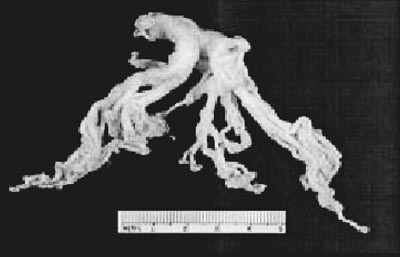
\includegraphics{./images/Image00057.jpg}
 \captionsetup{justification=centering}
 \caption{重症支气管哮喘患者形成的树状黏液栓}
 \label{fig7-1}
  \end{figure} 

\subsubsection{重症哮喘产生动态肺过度充气的原因是什么?}

重症哮喘产生动态肺过度充气是多种因素综合作用的结果。首先,呼气阻力增加使得呼气困难、呼气时间延长;其次,因低氧血症和(或)高碳酸血症可能导致呼吸驱动增加,从而增加呼吸频率、缩短呼气时间;第三,由于存在高碳酸血症,临床医生可能会通过增加潮气量和呼吸频率来增加肺泡通气量,以缓解高碳酸血症,而高的潮气量和快的呼吸频率会带来气道峰压和气道平台压增高、呼气时间缩短、产生呼气末气体在肺内的存留,即动态肺过度充气。重症哮喘动态肺过度充气的程度可以很严重。一项研究估计,重症哮喘患者“陷闭气体”的量可比正常呼气末容积高12~20ml/kg。

\subsubsection{重症哮喘发生呼吸衰竭的主要机制是什么?}

重症哮喘发生呼吸衰竭主要有两个机制。首先,弥漫、多变的支气管阻塞,导致通气血流比例失调而产生低氧血症,肺泡通气量不足可产生高碳酸血症;其次是呼吸肌疲劳,而吸气肌的疲劳比呼气肌更明显。因为哮喘的气道阻塞位于胸腔内,呼气相时气道狭窄更明显,使得呼气做功、呼气时间延长。然而,低氧血症、高碳酸血症和一些其他的因素,使得哮喘患者的呼吸驱动增加,呼吸频率增快、呼气时间缩短。明显呼气相气道梗阻、呼气时间缩短导致肺的过度充气。肺的过度充气使得吸气肌的负荷增加,吸气肌在收缩之前比正常时短,因此不能在同等时间内产生同等的张力。当不能代偿这种病理生理上的改变时即产生了呼吸衰竭。最终吸气肌疲劳、加重高碳酸血症和呼吸性酸中毒,常需要气管插管和机械通气。

\subsubsection{重症哮喘患者的治疗应遵循哪些原则?}

(1)氧疗 重症哮喘常由于通气/血流比失调导致不同程度的低氧血症,因此原则上应及时给予吸氧治疗。吸氧流量为1~3L/分钟,吸氧浓度一般不超过40%,维持经皮指脉氧饱和度>90%即可。普通氧疗后氧合改善仍不明显的患者,可考虑给予机械辅助通气治疗。此外,为避免气道干燥,吸入的氧气应经过加温加湿。

(2)解除支气管痉挛 对于重症哮喘患者不宜经口服或直接定量雾化吸入装置(MDI)给药,因为此时病人无法深吸气、屏气,也不能协调喷药与呼吸同步。可供选择的给药方式包括:①借助储雾器使用定量雾化吸入装置给药;②以高压氧气为动力,雾化吸入β\textsubscript{2}
受体激动剂或(和)抗胆碱能药物。一般情况下,成人每次雾化吸入喘乐宁1~2ml(含沙丁胺醇5~10mg),每日3~4次;③氨茶碱0.25g加入100ml葡萄糖液中30分钟静脉滴注完毕,继后予以氨茶碱0.5g加入葡萄糖液中持续静脉滴注,建议成人每日氨茶碱总量一般不超过1~1.5g。对于老年人、幼儿及肝肾功能障碍、甲亢或同时使用甲氰咪呱、喹诺酮或大环内酯类抗生素等药物者,应监测氨茶碱血药浓度。

(3)糖皮质激素的应用 一旦确诊为重症哮喘,在应用支气管解痉剂的同时,应及时足量地从静脉快速给予糖皮质激素,建议使用琥珀酸氢化可的松(因为该药为水溶制剂)(400~1000mg/天)或甲基泼尼松龙(160~240mg/天)。地塞米松抗炎作用较强,但由于在血浆和组织中半衰期长,对脑垂体肾上腺轴的抑制时间长,故应短时间使用或尽量避免使用。另外,吸入激素和吸入β\textsubscript{2}
受体激动剂可联合应用,治疗中、重度急性加重的哮喘患者。

(4)纠正脱水 重症哮喘由于存在摄水量不足,加之过度呼吸及出汗,常存在不同程度的脱水,导致气道分泌物黏稠,痰液难以排出,影响通气,因此补液有助于纠正脱水,稀释痰液,防止黏液栓形成。一般每日输液3000~4000ml,通常初始治疗时所需补液量往往较大,可根据临床监测情况决定补液量。

(5)积极纠正酸碱失衡和电解质紊乱 重症哮喘时,由于缺氧、过度消耗和入量不足等原因易于出现代谢性酸中毒,而在酸性环境下,许多支气管扩张剂不能充分发挥作用,故及时纠正酸中毒非常重要。建议在动脉血pH<7.2时可使用碱性药物。如果要立即实施机械通气,补碱应慎重,以避免过度通气造成呼吸性碱中毒。由于进食不佳和缺氧造成的胃肠道反应,患者常伴呕吐,并出现低钾、低氯性碱中毒,应予以补充。

(6)针对诱发发作的因素和并发症或伴发症进行预防及处理 如及时脱离致敏环境;对于感染导致哮喘加重的患者,应积极地抗感染治疗,包括合理使用抗生素。当然,除非有证据表明患者可能存在肺部细菌性感染,否则不提倡常规应用抗生素。另外,对重症哮喘并发症或伴发症(如心律失常、颅内高压、脑水肿、消化道出血等)也应注意预防并及时处理。

(7)硫酸镁 其作用机理不明确,可能与降低细胞内钙浓度致气道平滑肌舒张及其镇静作用有关。一般可在20分钟内静脉推注2g硫酸镁,也可与支气管扩张剂联合雾化吸入。

\subsubsection{如何评价无创正压通气在重症哮喘中的治疗地位?}

经氧疗及全身应用激素、雾化吸入β\textsubscript{2}
激动剂等药物治疗后,病情仍持续恶化,出现神志改变、呼吸肌疲劳、血气分析动脉血二氧化碳分压由低于正常转为正常或高于45mmHg者,需考虑机械辅助通气。

重症哮喘患者应用无创正压通气的时机目前尚无统一的标准
\protect\hyperlink{text00013.htmlux5cux23ch13-12}{\textsuperscript{{[}13{]}}}
。鉴于无创正压通气的并发症少,对于尚未达到插管上机标准的重症患者,尤其是伴有二氧化碳潴留而又无明显使用无创正压通气的禁忌证者,早期使用无创正压通气对于改善病人的病理生理状况,避免插管可能有积极的意义
\protect\hyperlink{text00013.htmlux5cux23ch14-12}{\textsuperscript{{[}14{]}}}
\textsuperscript{~}
\protect\hyperlink{text00013.htmlux5cux23ch16-12}{\textsuperscript{{[}16{]}}}
。可在严密监测的条件下试用无创正压通气1~2小时,若病情有恶化趋势,需尽早改为有创正压通气。虽然国内有个案报道
\protect\hyperlink{text00013.htmlux5cux23ch17-12}{\textsuperscript{{[}17{]}}}
,在病情非常危重的哮喘患者中应用无创正压通气,但由于无创正压通气的通气效果不如有创通气可靠,监测功能不完善,加之哮喘病人本身所需的通气时间较短,为避免延误病情,及早气管插管实施有创机械通气可能更为安全、有效。

\subsubsection{重症哮喘患者应用有创正压通气的指征是什么?}

重症哮喘患者行有创通气的绝对适应证为心跳呼吸骤停、呼吸浅快、意识不清或昏迷等。一般适应证为具有重症哮喘临床表现,特别是动脉血二氧化碳分压进行性升高伴酸中毒者。如动脉血二氧化碳分压>45mmHg,又具有下列情况之一则可考虑有创机械通气:①以前因哮喘严重发作而致呼吸停止、曾气管插管者;②以往有哮喘持续状态史,在使用糖皮质激素的情况下,此次又再发严重哮喘持续状态者。

为避免因延误治疗时机而导致的严重并发症,在医疗条件允许的情况下,气管插管实施有创机械通气宜早不宜迟,当患者出现呼吸肌疲劳的迹象,估计动脉血二氧化碳分压开始超过患者基础动脉血二氧化碳分压值时,就应准备气管插管。若经积极治疗无效,患者出现极度呼吸肌疲劳、低血压、心律失常、神志异常,应建立人工气道。一般选择经口气管插管,因为经口气管插管管径大、气道阻力小,便于痰液的引流和纤维支气管镜的操作。

\subsubsection{重症哮喘患者进行有创通气时,呼吸机参数应如何设置?}

重症哮喘患者在机械通气前已存在严重的呼吸肌疲劳,因此,机械通气早期可采用控制通气模式,使呼吸肌能得到充分休息,一旦患者自主呼吸功能有所恢复,需尽早改为辅助通气模式。

有创机械通气早期,呼吸机参数可按如下设置:潮气量5~7ml/kg,频率12~20次/分钟,呼气末正压<5cm
H\textsubscript{2} O(1cm H\textsubscript{2}
O=0.098kPa),调整吸气流速以延长呼气时间,保证吸呼比<1∶2,尽可能保持吸气末平台压<30~35cm
H\textsubscript{2} O,气道峰压<40cm H\textsubscript{2} O。

呼气未正压在哮喘患者中的应用仍存在着很大争议。呼气末正压使呼气状态肺泡内压增大,影响肺循环,而功能残气量增加,影响胸腔内压和体循环。对有严重气流受阻的重症哮喘,应用呼气末正压是有害的,可造成吸气末的肺容积明显增加,加重肺过度膨胀。对于气流受阻相对较轻,并且具有自主呼吸的患者,给予低水平呼气末正压(3~8cm
H\textsubscript{2} O,或不超过内源性呼气末正压),则可能从中受益。

一旦气道阻力开始下降以及动脉血二氧化碳分压恢复正常,镇静药及肌松剂已撤除,症状也明显好转,则应考虑撤机。

\subsubsection{无泵的动、静脉体外肺辅助系统在重症哮喘患者中有何应用价值?}

无泵的动、静脉体外肺辅助系统(pump-less arteriovenous extracorporeal
lung assist
system,pECLA)利用患者自身的股动、静脉压差将动脉血泵入低阻力的中空纤维气体交换膜内,进行气体交换后在动、静脉压差作用下重新流回体内
\protect\hyperlink{text00013.htmlux5cux23ch18-12}{\textsuperscript{{[}18{]}}}
。对降低血中二氧化碳水平具有较好的效果,因此,近年有学者开始将此系统应用于难治性哮喘患者,以治疗高碳酸血症。病例报告研究
\protect\hyperlink{text00013.htmlux5cux23ch19-12}{\textsuperscript{{[}19{]}}}
\textsuperscript{,}
\protect\hyperlink{text00013.htmlux5cux23ch20-12}{\textsuperscript{{[}20{]}}}
均显示,此系统能显著改善哮喘患者的高碳酸血症和酸中毒,并能降低呼吸机支持水平。因此,该治疗方法可能有助于降低呼吸机相关肺损伤发生的风险,但仍需临床随机对照研究进行证实。

\subsubsection{如何评价镇静剂和肌松剂在重症哮喘治疗中的作用?}

重症哮喘患者在气管插管或气管切开行机械通气时,应重视镇静及肌松剂的应用。镇静剂能给患者以舒适感,减少呼吸不同步,降低氧耗和二氧化碳的产生及内源性呼气末正压。常用的镇静药物有咪唑安定和异丙酚等。与地西泮(安定)比较,咪唑安定是一种快速和相对短效的苯二氮䓬
类药物,注射部位疼痛和血管刺激少,可比地西泮产生更舒适的催眠作用,同时产生明显的抗焦虑作用。咪唑安定达到中枢峰效应的时间为2~4分钟,其消除半衰期约2小时,多采用连续输注给药,先静脉推注负荷量0.025~0.05mg/kg后,以每分钟1.0~2.0μg/kg维持。异丙酚具有起效快、镇静过程平稳、不良反应少、镇静水平易于调节等优点,此外,该药还有一定的支气管扩张作用。一般可持续输注给药,约每分钟10~50μg/kg,并根据患者镇静状态进行调节。

肌松剂虽具有避免人机对抗、减少气压伤及降低呼吸功耗等优点,但亦会伴有严重的副作用,如肌病、分泌物产生增多、组胺释放增加、心动过速和低血压等。特别是在合并使用大剂量糖皮质激素治疗时,肌松剂的应用可能会增加肌病的发生率。所以,对于重症哮喘患者应尽量减少肌松剂的使用,除非在充分镇静后,仍存在人机不协调,频繁气道高压报警,甚至出现动脉氧分压下降等情况,可考虑使用小剂量肌松剂。

\begin{center}\rule{0.5\linewidth}{\linethickness}\end{center}

参考文献

\protect\hyperlink{text00013.htmlux5cux23ch1-12-back}{{[}1{]}} .Rodrigo
G,Rodrigo C.Corticosteroids in the emergency department therapy of
adult acute asthma treatment:an evidence based
evaluation.Chest,2002,121:1977-1987.

\protect\hyperlink{text00013.htmlux5cux23ch2-12-back}{{[}2{]}} .Foresi
A,Paggiaro P.Inhaled corticosteroids and leukotriene modifiers in the
acute treatment of asthma exacerbations.Cur Opin Pul
Med,2003,9:52-56.

\protect\hyperlink{text00013.htmlux5cux23ch3-12-back}{{[}3{]}}
.Brocklebank D,Wright J,Cates C.Systematic review of clinical
effectiveness of pressurised metered dose inhalers versus other hand
held inhaler devices for delivering corticosteroids in
asthma.BMJ,2001,323:896-900.

\protect\hyperlink{text00013.htmlux5cux23ch4-12-back}{{[}4{]}}
.Anderson PB,Langley SJ,Mooney P,et al.Equivalent efficacy and
safety of a new HFA-134a formulation of BDP compared with the
conventional CFC in adult asthmatics.J Investig Allergol Clin
Immunol,2002,12:107-113.

\protect\hyperlink{text00013.htmlux5cux23ch5-12-back}{{[}5{]}}
.Boonsawat W,Charoenratanakul S,Pothirat C,et
al.Formoterol(OXIS)Turbuhaler as a rescue therapy compared with
salbutamol pMDI plus spacer in patients with acute severe asthma.Respir
Med,2003,97:1067-1074.

\protect\hyperlink{text00013.htmlux5cux23ch6-12-back}{{[}6{]}}
.Hospenthal MA,Peters JI.Long-acting beta(2)-agonists in the
management of asthma exacerbations.Curr Opin Pulm
Med,2005,11:69-73.

\protect\hyperlink{text00013.htmlux5cux23ch7-12-back}{{[}7{]}} .Salo
D,Tuel M,Lavery RF,et al.A randomized,clinical trial comparing the
efficacy of continuous nebulized albuterol(15 mg)versus continuous
nebulized albuterol(15 mg)plus ipratropium bromide(2 mg)for the
treatment of acute asthma.J Emerg Med,2006,31:371-376.

\protect\hyperlink{text00013.htmlux5cux23ch8-12-back}{{[}8{]}}
.Yamauchi K,Kobayashi H,Tanifuji Y,et al.Efficacy and safety of
intravenous theophylline administration for treatment of mild acute
exacerbation of bronchial asthma.Respirology,2005,10:491-496.

\protect\hyperlink{text00013.htmlux5cux23ch9-12-back}{{[}9{]}} .Blitz
M,Blitz S,Hughes R,et al.Aerosolized Magnesium Sulfate for Acute
Asthma:A Systematic Review.Chest,2005,128:337-344.

\protect\hyperlink{text00013.htmlux5cux23ch10-12-back}{{[}10{]}} .Blitz
M,Blitz S,Beasely R,et al.Inhaled magnesium sulfate in the treatment
of acute asthma.Cochrane Database Syst Rev,2005,19:CD003898.

\protect\hyperlink{text00013.htmlux5cux23ch11-12-back}{{[}11{]}}
.Piatti G,Ceriotti L,Cavallaro G.Effects of zafirlukast on bronchial
asthma and allergic rhinitis.Pharmacological
research,2003,6:541-547.

\protect\hyperlink{text00013.htmlux5cux23ch12-12-back}{{[}12{]}}
.Silverman RA,Nowak RM,Korenblat PE,et al.Zafirlukast treatment for
acute asthma:evaluation in a randomized,double-blind,multicenter
trial.Chest,2004,126:1480-1489.

\protect\hyperlink{text00013.htmlux5cux23ch13-12-back}{{[}13{]}} .Ram
FS,Wellington S,Rowe B,et al.Non-invasive positive pressure
ventilation for treatment of respiratory failure due to severe acute
exacerbations of asthma.Cochrane Database Syst
Rev.2005,20:CD004360.

\protect\hyperlink{text00013.htmlux5cux23ch14-12-back}{{[}14{]}}
.Meduri GU,Cook TR,Turner RE,et al.Noninvasive positive pressure
ventilation in status asthmaticus.Chest,1996,110:767-774.

{[}15{]}.Fernandez MM,Villagra A,Blanch L,et al.Non-invasive
mechanical ventilation in status asthmaticus.Intensive Care
Med,2001,27:486-492.

\protect\hyperlink{text00013.htmlux5cux23ch16-12-back}{{[}16{]}}
.詹庆元,刘利,王辰.无创正压通气治疗急性重症支气管哮喘.中华结核和呼吸杂志,2004,27:132-133.

\protect\hyperlink{text00013.htmlux5cux23ch17-12-back}{{[}17{]}}
.钮善福,朱蕾.危重支气管哮喘治疗体会.中华结核和呼吸杂志,1998,21:372-373.

\protect\hyperlink{text00013.htmlux5cux23ch18-12-back}{{[}18{]}}
.Muller T,Lubnow M,Philipp A,et al.Extracorporeal pumpless
interventional lung assist in clinical practice:determinants of
efficacy.Eur Respir J,2009,33(3):551-558.

\protect\hyperlink{text00013.htmlux5cux23ch19-12-back}{{[}19{]}} .Twigg
S,Gibbon GJ,Perris T.The use of extracorporeal carbon dioxide removal
in the management of life-threatening bronchospasm due to influenza
infection.Anaesth Intensive Care,2008,36(4):579-581.

\protect\hyperlink{text00013.htmlux5cux23ch20-12-back}{{[}20{]}}
.Elliot SC,Paramasivam K,Oram J,et al.Pumpless extracorporeal
carbon dioxide removal for life-threatening asthma.Crit Care
Med,2007,35(3):945-948.

\protect\hypertarget{text00014.html}{}{}

